\noindent
\begin{minipage}[t]{0.33\textwidth}
\textbf{69.}\enspace Cho bảng giá trị của $f$, $g$, $f'$ và $g'$:
\vspace{0.3em}
\begin{center}
\footnotesize
\renewcommand{\arraystretch}{1.15}
\begin{tabular}{|c|c|c|c|c|}
\hline
\rowcolor{tableheader}
$x$ & $f(x)$ & $g(x)$ & $f'(x)$ & $g'(x)$ \\
\hline
$1$ & $3$ & $2$ & $4$ & $6$ \\
$2$ & $1$ & $8$ & $5$ & $7$ \\
$3$ & $7$ & $2$ & $7$ & $9$ \\
\hline
\end{tabular}
\end{center}
\vspace{0.2em}
\textbf{(a)}\enspace Nếu $h(x) = f(g(x))$, hãy tìm $h'(1)$.\\[0.25em]
\textbf{(b)}\enspace Nếu $H(x) = g(f(x))$, hãy tìm $H'(1)$.

\vspace{0.7em}
\textbf{70.}\enspace Cho $f$ và $g$ là các hàm số trong Bài tập 69.\\[0.25em]
\textbf{(a)}\enspace Nếu $F(x) = f(f(x))$, hãy tìm $F'(2)$.\\[0.25em]
\textbf{(b)}\enspace Nếu $G(x) = g(g(x))$, hãy tìm $G'(3)$.

\vspace{0.7em}
\textbf{71.}\enspace Nếu $f$ và $g$ là các hàm số có đồ thị như hình vẽ, đặt $u(x) = f(g(x))$, $v(x) = g(f(x))$ và $w(x) = g(g(x))$. Hãy tìm mỗi đạo hàm sau nếu nó tồn tại. Nếu không tồn tại, hãy giải thích tại sao.\\[0.25em]
\textbf{(a)}\enspace $u'(1)$ \quad \textbf{(b)}\enspace $v'(1)$ \quad \textbf{(c)}\enspace $w'(1)$
\begin{center}
\vspace{0.2em}
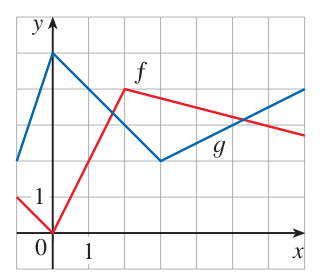
\includegraphics[width=0.88\linewidth]{images/p0242_fig1.png}
\end{center}

\vspace{0.4em}
\textbf{72.}\enspace Nếu $f$ là hàm số có đồ thị như hình vẽ, đặt $h(x) = f(f(x))$ và $g(x) = f(x^2)$. Hãy sử dụng đồ thị của $f$ để ước lượng giá trị của mỗi đạo hàm sau.\\[0.25em]
\textbf{(a)}\enspace $h'(2)$ \qquad\qquad \textbf{(b)}\enspace $g'(2)$
\begin{center}
\vspace{0.2em}
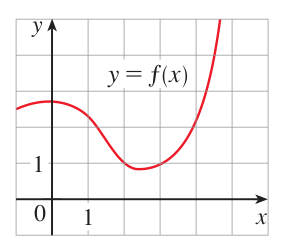
\includegraphics[width=0.85\linewidth]{images/p0242_fig2.png}
\end{center}

\vspace{0.4em}
\textbf{73.}\enspace Nếu $g(x) = \sqrt{f(x)}$, trong đó đồ thị của $f$ được cho như hình bên, hãy tính $g'(3)$.
\begin{center}
\vspace{0.2em}
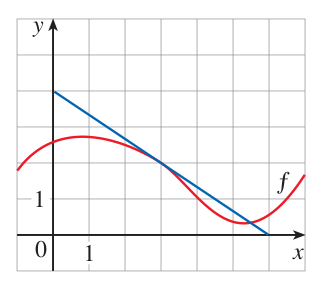
\includegraphics[width=0.85\linewidth]{images/p0242_fig3.png}
\end{center}
\end{minipage}%
\hfill
\begin{minipage}[t]{0.64\textwidth}
\textbf{74.}\enspace Giả sử $f$ khả vi trên $\mathbb{R}$ và $\alpha$ là một số thực. Đặt $F(x) = f(x^\alpha)$ và $G(x) = [f(x)]^\alpha$. Tìm biểu thức cho \textbf{(a)} $F'(x)$ và \textbf{(b)} $G'(x)$.

\vspace{0.65em}
\textbf{75.}\enspace Giả sử $f$ khả vi trên $\mathbb{R}$. Đặt $F(x) = f(e^x)$ và $G(x) = e^{f(x)}$. Tìm biểu thức cho \textbf{(a)} $F'(x)$ và \textbf{(b)} $G'(x)$.

\vspace{0.65em}
\textbf{76.}\enspace Cho $g(x) = e^{cx} + f(x)$ và $h(x) = e^{kx}f(x)$, trong đó $f(0) = 3$, $f'(0) = 5$ và $f''(0) = -2$.\\[0.2em]
\textbf{(a)}\enspace Tìm $g'(0)$ và $g''(0)$ theo $c$.\\[0.2em]
\textbf{(b)}\enspace Theo $k$, hãy tìm phương trình tiếp tuyến của đồ thị hàm số $h$ tại điểm có $x = 0$.

\vspace{0.65em}
\textbf{77.}\enspace Cho $r(x) = f(g(h(x)))$, trong đó $h(1) = 2$, $g(2) = 3$, $h'(1) = 4$, $g'(2) = 5$ và $f'(3) = 6$. Tìm $r'(1)$.

\vspace{0.65em}
\textbf{78.}\enspace Nếu $g$ là một hàm số khả vi hai lần và $f(x) = xg(x^2)$, hãy tìm $f''$ theo $g$, $g'$ và $g''$.

\vspace{0.65em}
\textbf{79.}\enspace Nếu $F(x) = f(3f(4f(x)))$, trong đó $f(0) = 0$ và $f'(0) = 2$, hãy tìm $F'(0)$.

\vspace{0.65em}
\textbf{80.}\enspace Nếu $F(x) = f(xf(xf(x)))$, trong đó $f(1) = 2$, $f(2) = 3$, $f'(1) = 4$, $f'(2) = 5$ và $f'(3) = 6$, hãy tìm $F'(1)$.

\vspace{0.65em}
\textbf{81.}\enspace Chứng minh rằng hàm số $y = e^{2x}(A\cos 3x + B\sin 3x)$ thỏa mãn phương trình vi phân $y'' - 4y' + 13y = 0$.

\vspace{0.65em}
\textbf{82.}\enspace Với các giá trị nào của $r$ thì hàm số $y = e^{rx}$ thỏa mãn phương trình vi phân $y'' - 4y' + y = 0$?

\vspace{0.65em}
\textbf{83.}\enspace Tìm đạo hàm cấp 50 của $y = \cos 2x$.

\vspace{0.65em}
\textbf{84.}\enspace Tìm đạo hàm cấp 1000 của $f(x) = xe^{-x}$.

\vspace{0.65em}
\textbf{85.}\enspace Độ dời của một chất điểm trên một sợi dây dao động được cho bởi phương trình
\[
s(t) = 10 + \frac{1}{4}\sin(10\pi t)
\]
trong đó $s$ tính bằng centimét và $t$ tính bằng giây. Tìm vận tốc của chất điểm sau $t$ giây.

\vspace{0.6em}
\textbf{86.}\enspace Nếu phương trình chuyển động của một chất điểm được cho bởi $s = A\cos(\omega t + \delta)$, chất điểm được gọi là dao động điều hòa đơn giản.\\[0.2em]
\textbf{(a)}\enspace Tìm vận tốc của chất điểm tại thời điểm $t$.\\[0.2em]
\textbf{(b)}\enspace Khi nào thì vận tốc bằng 0?

\vspace{0.6em}
\textbf{87.}\enspace Sao biến quang Cepheid là một ngôi sao có độ sáng luân phiên tăng và giảm. Ngôi sao dễ quan sát nhất thuộc loại này là Delta Cephei, có chu kỳ giữa các lần đạt cực đại độ sáng là $5{,}4$ ngày. Độ sáng trung bình của ngôi sao này là $4{,}0$ và độ sáng của nó biến thiên $\pm 0{,}35$. Dựa trên các dữ liệu này, độ sáng của Delta Cephei tại thời điểm $t$, trong đó $t$ tính bằng ngày, được mô hình hóa bởi hàm số
\[
B(t) = 4{,}0 + 0{,}35\sin\left(\frac{2\pi t}{5{,}4}\right)
\]
\textbf{(a)}\enspace Tìm tốc độ biến thiên của độ sáng sau $t$ ngày.\\[0.2em]
\textbf{(b)}\enspace Tìm tốc độ tăng độ sáng sau một ngày, chính xác đến hai chữ số thập phân.
\end{minipage}

\vfill
\begin{center}
\fontsize{6.5pt}{8pt}\selectfont\color{copyrightgray}
Copyright 2021 Cengage Learning. All Rights Reserved. May not be copied, scanned, or duplicated, in whole or in part. WCN 02-200-203\\
Editorial review has deemed that any suppressed content does not materially affect the overall learning experience. Cengage Learning reserves the right to remove additional content at any time if subsequent rights restrictions require it.
\end{center}
